\SubSection{GPU Baseline Results}

In this section, we elaborate on the benchmarking deep neural networks that we choose, then we run them in 3 kinds of GPU frequencies to obtain the power, performance, and temperature profiles. These profiles act as the baseline for the study of the CPU-GPU execution scenario.

\paragraph{Benchmarks}

We choose small, medium, and large deep neural networks in terms of the depth of the network. Specifically, we choose 3 neural networks from those that are used to tackle image classification task of the ImageNet dataset. We summarize the benchmark we choose in Table.~\ref{table:1}. We measure the memory overhead by using \textit{tegrastat} provided by NVIDIA while inferencing the image.

Notice that there is only 4GB of RAM available on TX1, which is shared between CPU and GPU, with 1GB reserved by the operating system (Ubuntu). Hence, in the case of ResNet-152, it almost consumes all the available memory of the system that might leave barely nothing for the CPU. On the other hand, the shallowest neural network we have is AlexNet, and it still consumes a large amount of memory, i.e. 720 MB.


\begin{table}[h]
    \begin{center}
        \begin{tabular}{ | c | c | c | c | }
        \hline
        & Memory (MB) & \# Layers & Top-1 Acc. \\ \hline
        AlexNet{\cite{krizhevsky2012imagenet}} & 720 & 7 & 57.2\% \\ \hline
        GoogLeNet{\cite{szegedy2015going}} & 820 & 22 & 68.7\%  \\ \hline
        ResNet-152{\cite{he2016deep}} & 2224 & 152 & 77.0\% \\
        \hline
        \end{tabular}
    \end{center}
    \caption{The descriptions of the deep neural networks we choose, including the memory overhead during inference (single image), number of layers, and the reported top-1 accuracy on ImageNet.}\label{table:1}
\end{table}

We choose 3 kinds of GPU voltage/frequency pairs, i.e. the smallest (0.82 V, 76.8 Mhz), the medium (0.85 V, 537.6 Mhz), and the largest (1.1 V, 998.4 Mhz), from the 13 available voltage and frequency pairs on NVIDIA Tegra X1 to further investigate the power, latency, and temperature profiles of the aforementioned benchmarks.

\paragraph{Profiling}

We sweep through 3 different voltage and frequency pairs for each of the benchmark that we study and collect the temperature of both CPU and GPU, the power consumption of the GPU, and the latency of the tasks.

\begin{figure}[h]
    \centering
    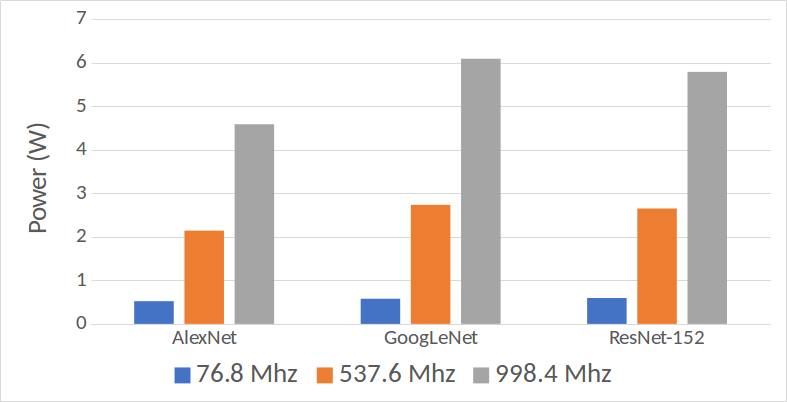
\includegraphics[width=0.5\textwidth]{power_profile.png}
    \caption{The power profile when running DNN benchmarks under different GPU voltage/frequency pairs.}\label{fig:1}
\end{figure}

\begin{figure}[h]
    \centering
    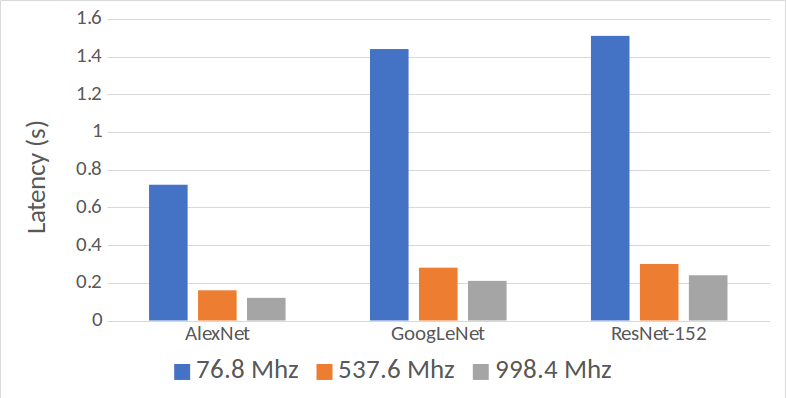
\includegraphics[width=0.5\textwidth]{latency_profile.png}
    \caption{The latency profile when running DNN benchmarks under different GPU voltage/frequency pairs.}\label{fig:2}
\end{figure}

Figure~\ref{fig:1} and Figure~\ref{fig:2} show both the power and latency profile of the aforementioned DNN benchmarks running under different GPU voltage/frequency pairs. As expected, the power consumption is higher when the GPU voltage and frequency are higher. Also, the deeper the neural network the higher the latency. Interestingly, the power consumption of GoogLeNet is higher than ResNet-152 at each voltage and frequency pair, which implies that the utilization of the GPU when running GoogLeNet is higher than ResNet-152. On the other hand, the three benchmarks share similar temperature profiles, i.e. around 40C on average, which is far from the throttling temperature of the GPU on TX1, i.e. 89.5C.

To further compare and analyze the characteristics of these benchmarks, we normalize the latency, power consumption, and accuracy to AlexNet as shown in Figure~\ref{fig:3}. From AlexNet to GoogLeNet, the major increase of the cost is latency and power consumption with slightly increase in memory overhead. Though at the first glance that accuracy improves from 57.2\% to 68.7\% is not much compared to the increment in cost, it is hard to judge the impact of accuracy on the quality of services. On the other hand, from GoogLeNet to ResNet-152, the major cost increase is memory, i.e. more than 2x. In terms of memory overhead and accuracy, it seems that it does not worth it to go from GoogLeNet to ResNet-152 unless there is a hard target for the accuracy since it requires much more memory with small accuracy improvement.

\begin{figure}[h]
    \centering
    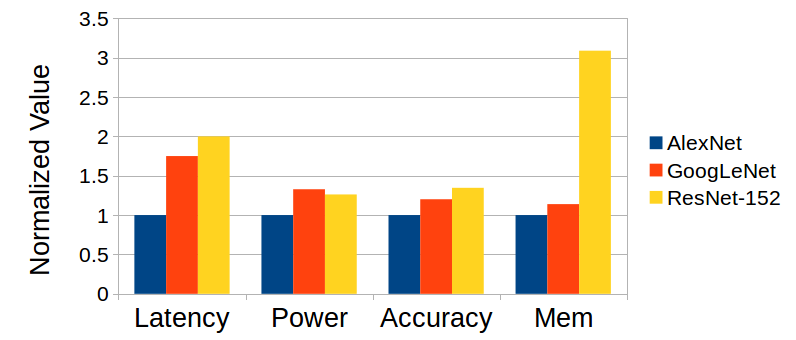
\includegraphics[width=0.5\textwidth]{benchmark_compare.png}
    \caption{Compare the benchmarks in terms of latency, power consumption, memory overhead, and accuracy. The values are normalized to AlexNet. We fix the voltage/frequency pair to the highest one.}\label{fig:3}
\end{figure}

\SubSection{CPU Baseline Results}

We choose 3 different benchmarks for CPU in MiBench benchmark suite. We run them in 3 CPU frequencies and obtain power, performance, and temperature results. These results provide baseline profiles for our final analysis in which we run CPU and GPU benchmarks together to better understand the trade-offs between various power and performance metrics.

\paragraph{Benchmarks}


We choose memory-intensive (jpeg), compute-intensive (bitcount), and a balanced (stringsearch) benchmarks from MiBench. In the previous report, we proposed to use SPLASH2 \cite{woo1995splash} benchmark suite. However, we changed it to MiBench and more daily usage benchmarks such as stringsearch which is an office benchmark. Our motivation to choose these benchmarks is doing meaningful work while running DNN on GPU. Hence, one may use CPU to run office programs while running a DNN inference on GPU. 

\begin{figure}
  \caption{Characteristics of chosen CPU benchmarks.}
  \centering
    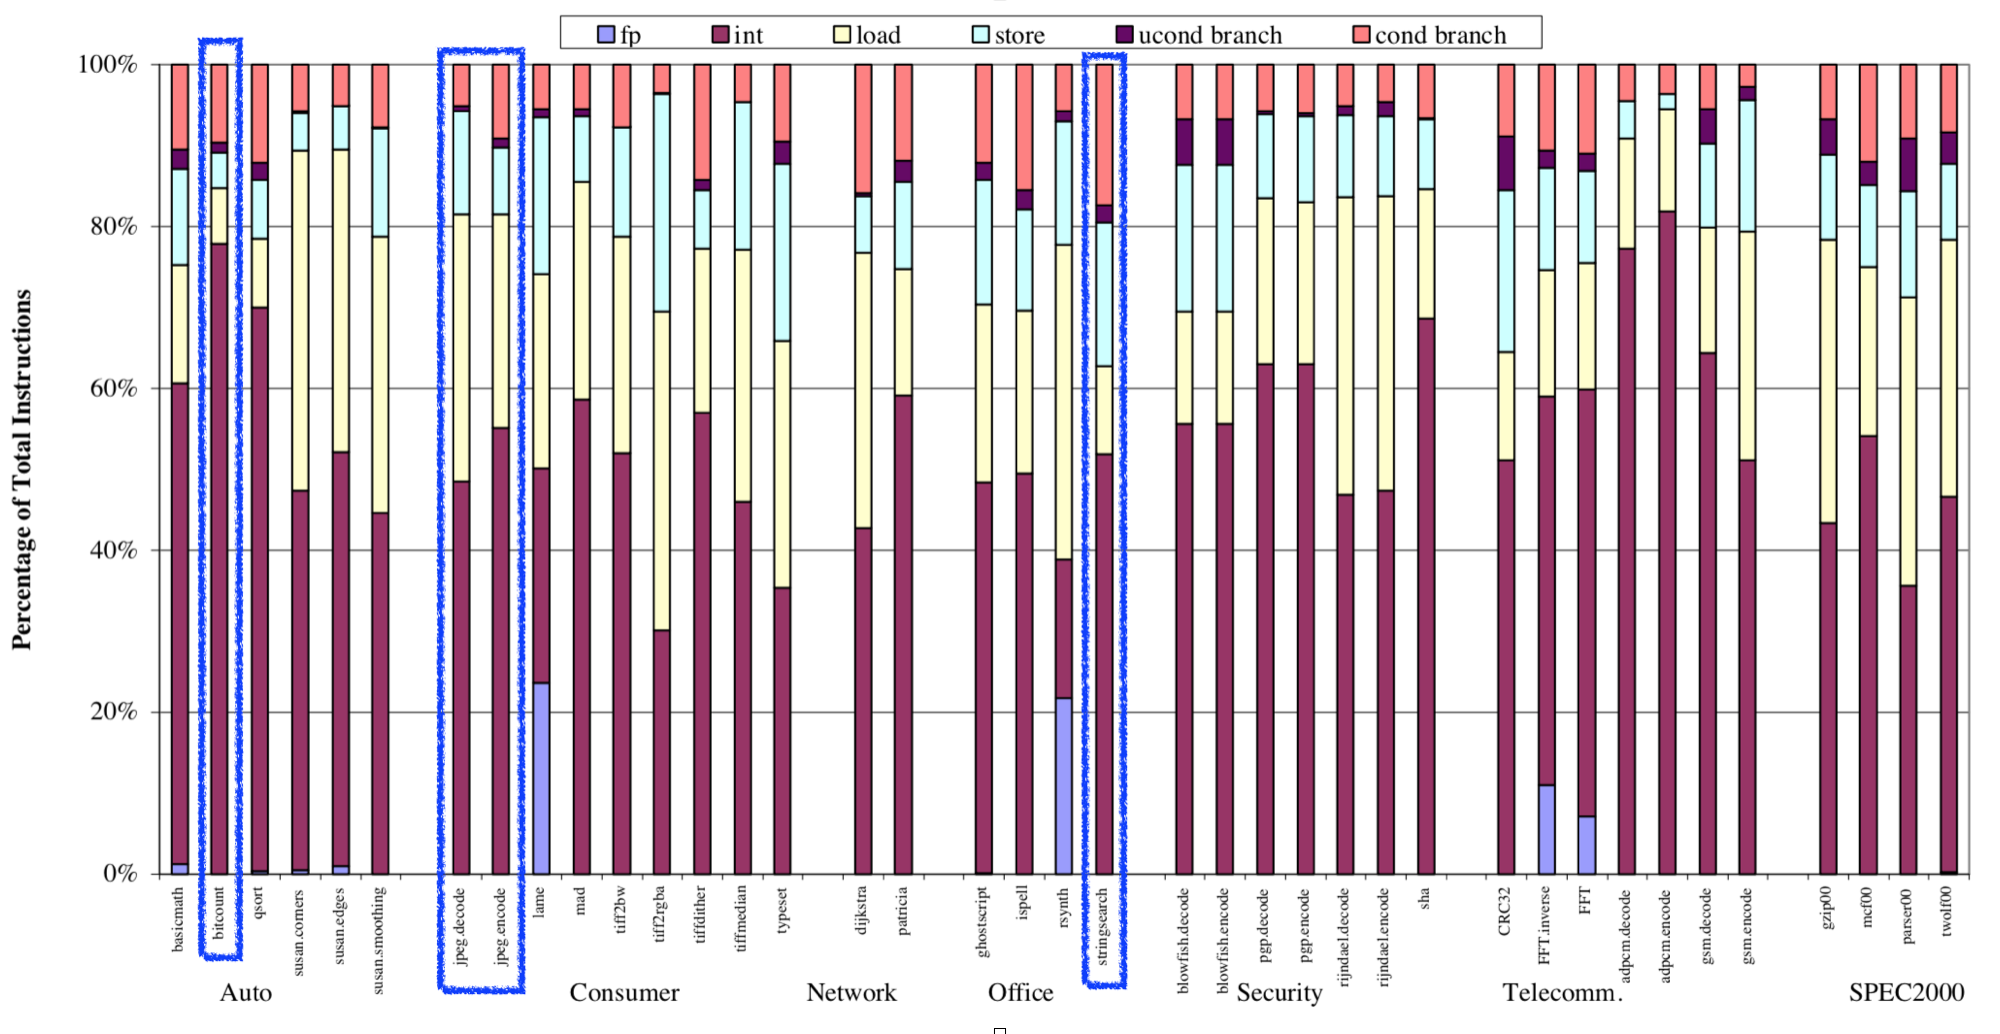
\includegraphics[width=0.5\textwidth]{cpubench}
\end{figure}

We run these benchmarks at 3 different frequency values which are the lowest (102 Mhz), the middle (921.6 Mhz), and the highest (1.73 Ghz) available frequency values for CPU. 

\paragraph{Profiling}


We run aforementioned 3 benchmarks with 3 different frequency values for CPU while not running anything on GPU to obtain a baseline for CPU. We calculate power, performance, and temperature results for CPU. 

\begin{figure}[h]
    \centering
    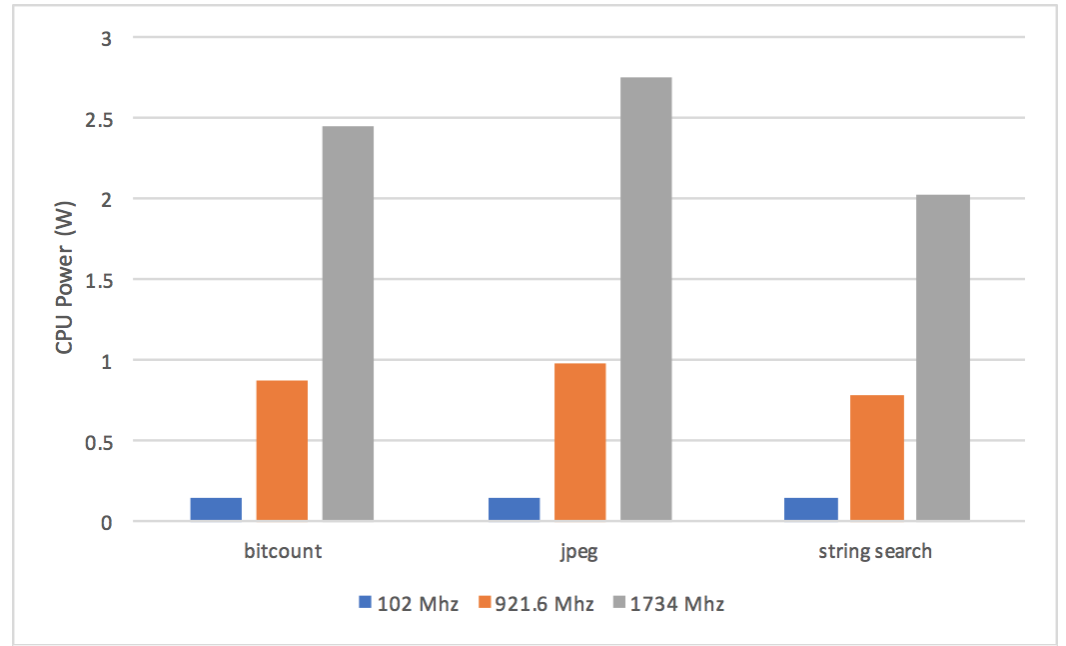
\includegraphics[width=0.5\textwidth]{cpupower.png}
    \caption{The power profile when running CPU benchmarks under different CPU voltage/frequency pairs.}\label{fig:cpupower}
\end{figure}

We calculate power consumption using sensors in TX1 board as it is shown in Figure 5. One of the observations is that power consumption increases as we increase CPU frequency. Another important observation is that power consumption is the highest for jpeg encode/decode benchmark which is an image compression and decompression workload. Furthermore, the lowest power consumption comes from stringsearch benchmark which is an office workload. 
Moreover, we calculate temperature (Celcius) by using thermal sensors in TX1 board. Figure 6. shows temperature profile of CPU and GPU while running CPU benchmarks with various frequency values. Temperature results also follow the same trend with power results. In addition, GPU temperature also follows the same trend with CPU temperature since GPU does not run anything and CPU temperature affects GPU temperature. 
We also obtain performance results by using instruction per cycle (IPC) metric and CPU utilization for each frequency and benchmark pairs. Figure 7. shows IPC and CPU utilization results for each benchmark and frequency values. Results show that IPC value does not change when we change frequency values. Furthermore, CPU utilization is also at almost 100\% for bitcount and jpeg benchmarks. However, CPU utilization is only 83\% at 102 Mhz and it becomes 44\% at 1.73 Ghz. It shows us that stringsearch benchmark does not need as much CPU resources as other benchmarks. 
Another significant conclusion is that IPC value of bitcount is higher than jpeg benchmark. However, power consumption of jpeg is higher than bitcount benchmark. It reveals that jpeg uses more power consuming instructions.


\begin{figure}[h]
    \centering
    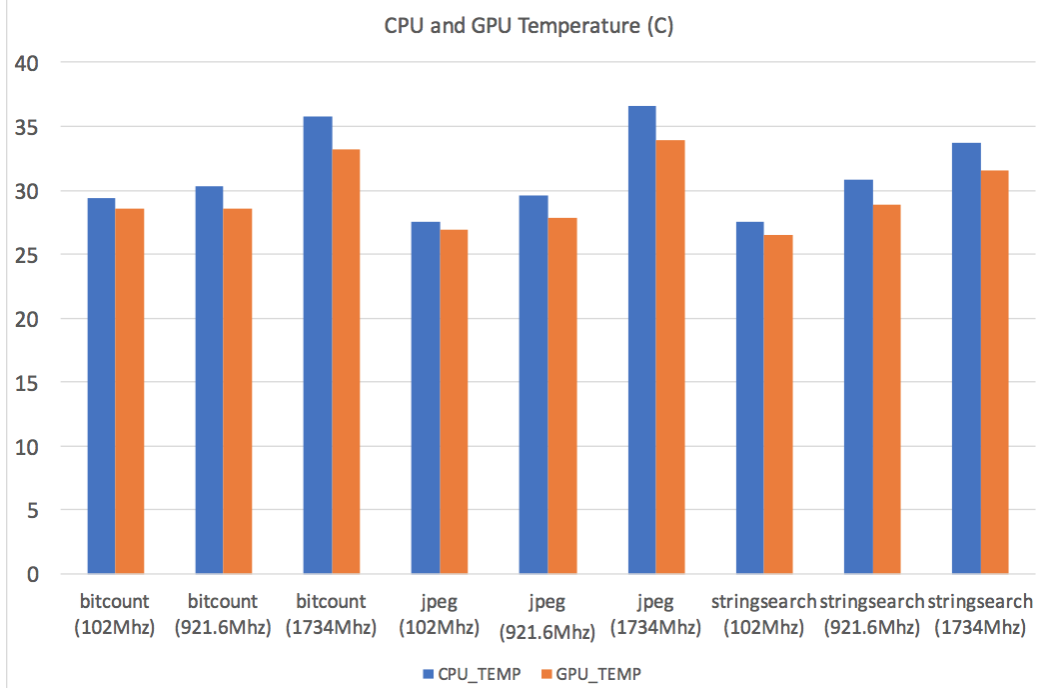
\includegraphics[width=0.5\textwidth]{cputemp.png}
    \caption{The temperature profile of CPU and GPU while running CPU benchmarks under different CPU voltage/frequency pairs.}\label{fig:cputemp}
\end{figure}


\begin{figure}[h]
    \centering
    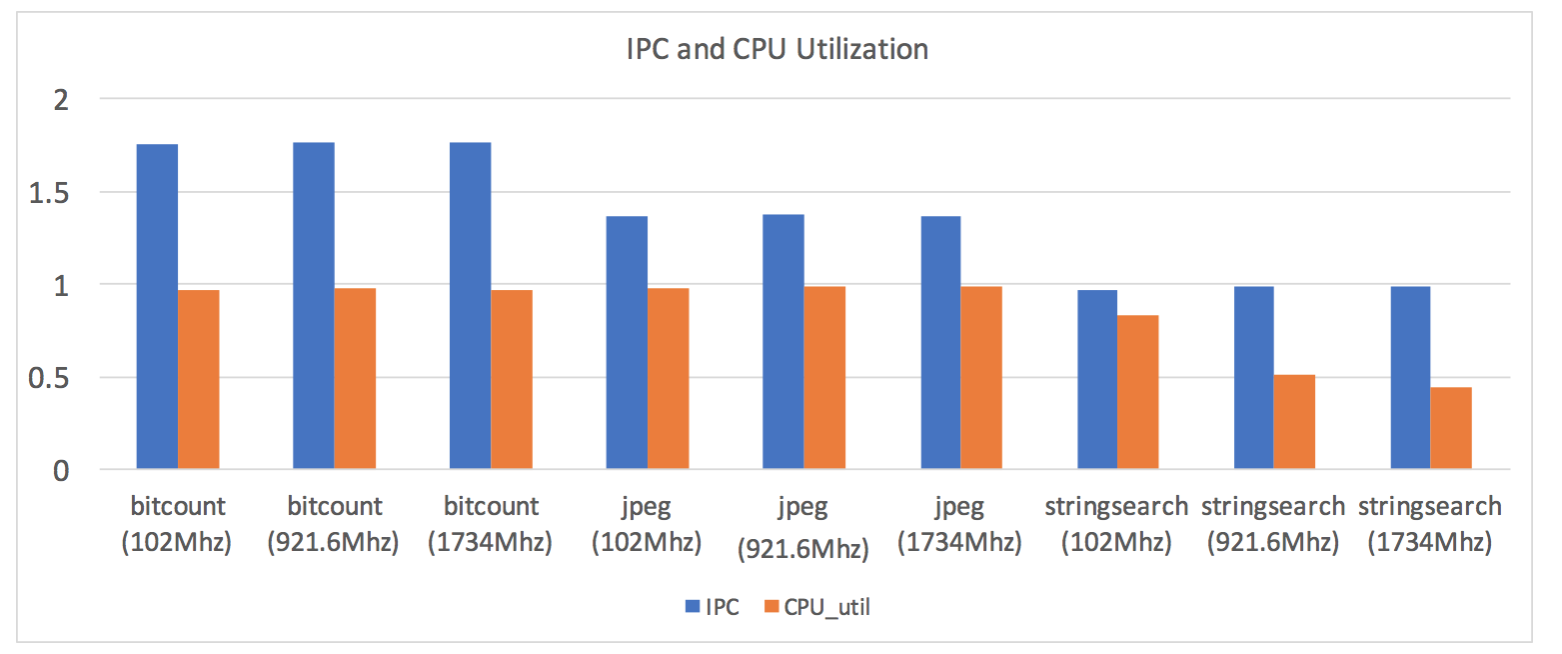
\includegraphics[width=0.5\textwidth]{cpuipc.png}
    \caption{The performance profile of CPU while running CPU benchmarks under different CPU voltage/frequency pairs.}\label{fig:cpuperf}
\end{figure}

\SubSection{CPU-GPU Results}

In this section, we analyze various power and performance metrics by running CPU and GPU benchmarks together. 


\begin{figure}[h]
    \centering
    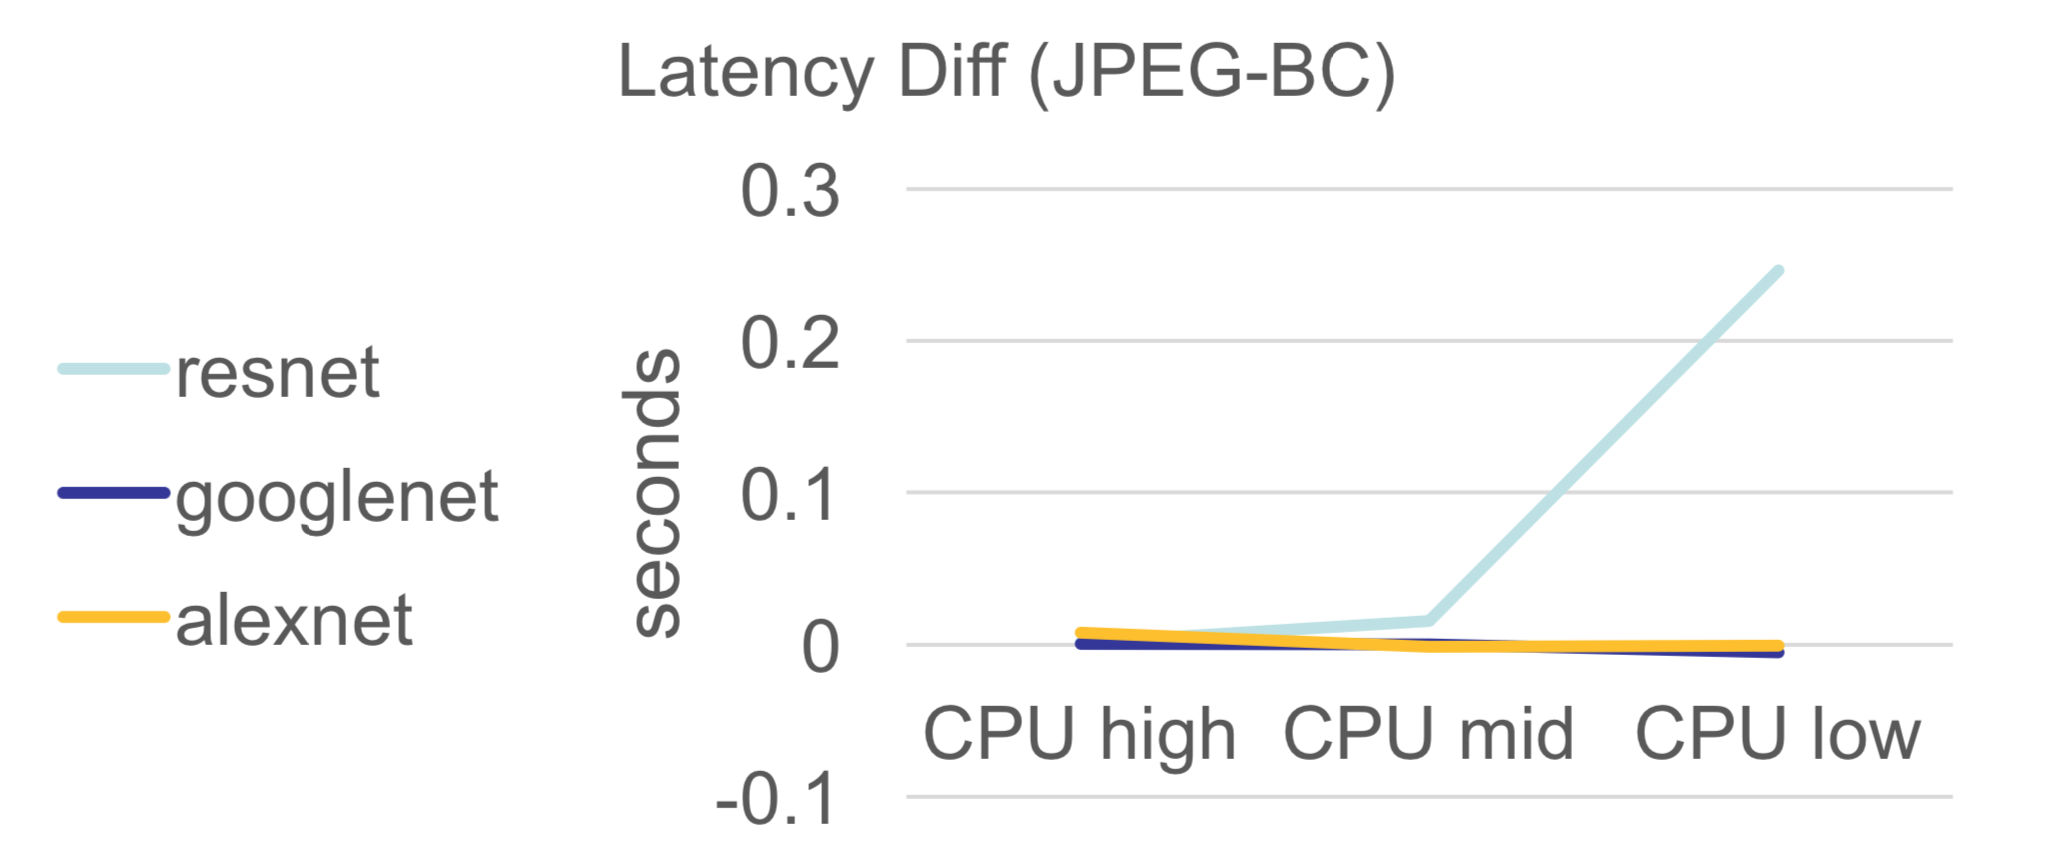
\includegraphics[width=0.5\textwidth]{latencydiff.png}
    \caption{The latency difference between jpeg and bitcount benchmarks for various DNNs by using various CPU frequency values}\label{fig:latencydiff}
\end{figure}


Figure~\ref{fig:latencydiff} shows the latency difference between a memory-intensive CPU benchmark (jpeg encode/decode) and a compute-intensive CPU benchmark (bitcount) for various DNNs by using high, mid, and low CPU frequency values. Results show that when we run memory-intensive DNNs such as ResNet, memory-intensive CPU benchmarks such as jpeg encode/decode adversely affects the DNN latency. We observe 13\% performance difference with ResNet compared to other DNNs. Hence, these results show that memory consumption of both DNN and CPU benchmarks plays an important role in overall power and performance. 

\begin{figure}[h]
    \centering
    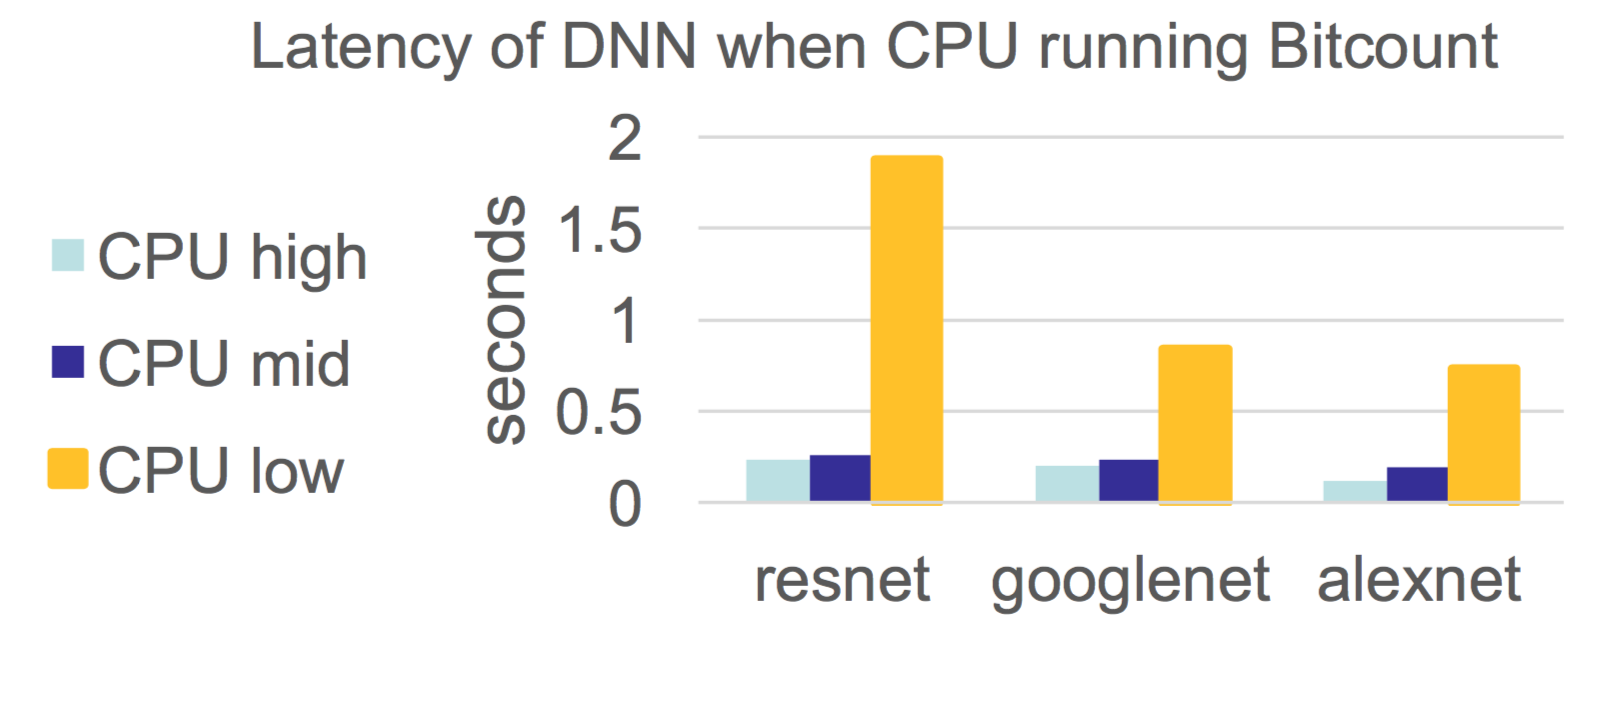
\includegraphics[width=0.5\textwidth]{latencycpu.png}
    \caption{The latency of various DNNs when CPU running bitcount benchmark with various CPU frequency values}\label{fig:latencycpu}
\end{figure}


Figure~\ref{fig:latencycpu} shows the latency of various DNNs when CPU running a compute-intensive (bitcount) benchmark by using high, mid, and low cpu frequency values. Results show that although most of the deep learning tasks can be run on GPU, frequency of CPU still plays an important role due to data preparation stage. We observe up to 8.2x performance difference with low CPU frequency and high CPU frequency configurations. This affect increases as we use larger DNNs such as ResNet. 

\begin{figure}[h]
    \centering
    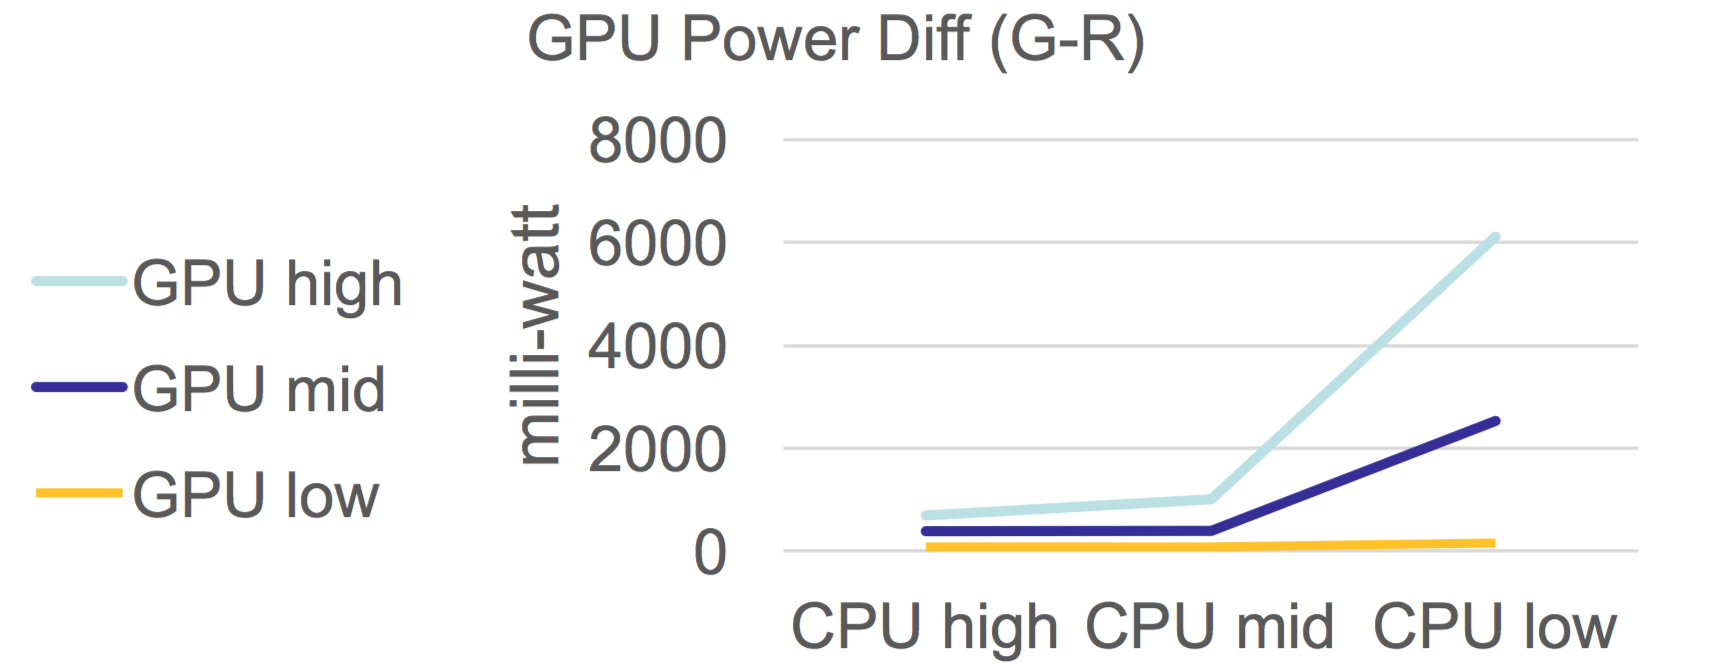
\includegraphics[width=0.5\textwidth]{gpupowerdiff.png}
    \caption{The GPU power consumption difference between GoogLeNet and ResNet by using various CPU and GPU frequency configurations}\label{fig:gpupowerdiff}
\end{figure}


Figure~\ref{fig:gpupowerdiff} shows the GPU power consumption difference between GoogLeNet and ResNet by using various CPU and GPU frequency configurations. It shows that GoogLeNet consumes more power than ResNet-152, which is deeper and larger, consistently. It exaggerates as the gap between CPU and GPU frequency values grows larger. 
